\documentclass{article}

\usepackage{fullpage}
\usepackage{amsmath}
\usepackage{amsfonts}
\usepackage{graphicx}
\usepackage{algorithmic}
\usepackage{xcolor}
\usepackage{framed}

\definecolor{dark_red}{rgb}{0.5,0.0,0.0}

\newcommand{\abs}[1]{\left|#1\right|}
\newcommand{\atan}{\text{atan}}
\newcommand{\rowvec}[3]{\left\langle #1, #2, #3 \right\rangle}
\newcommand{\colvec}[3]{\begin{bmatrix} #1 \\ #2 \\ #3 \end{bmatrix}}
\newcommand{\at}[1]{\left. #1 \right|}
\newcommand{\diff}[2]{\frac{d #1}{d #2}}
\newcommand{\partdiff}[2]{\frac{\partial #1}{\partial #2}}
\newcommand{\mvec}[1]{\overrightarrow{\mathbf{#1}}}
\newcommand{\pvec}[1]{\overrightarrow{#1}}
\newcommand{\dr}[1]{\textcolor{dark_red}{#1}}


\title{Double and Triple Integrals}
\date{}

\begin{document}

\maketitle



%%%%%%%%%%%%%% QUESTION 1
\section*{Question 1:}

Find the minimum and maximum values of the function:
\[f(x,y) = x + y\]
subject to the constraint:
\[x^2 + 4y^2 - 4x - 16y = -16\] 



%%%%%%%%%%%%%% QUESTION 2
\section*{Question 2:}

Find the minimum and maximum values of the function:
\[f(x,y) = 2x + y\]
subject to the constraint:
\[x^2 + y^2 - 2x - 2y = 2\]



%%%%%%%%%%%%%% QUESTION 3
\section*{Question 3:}

\begin{tabular}{cc}
\parbox{0.6\textwidth}{The leaf shaped region \(\sigma\) on the right is bounded from below by a parabola and from above by a straight line. Express \(\sigma\) as a Type I Cartesian region; a Type II Cartesian region; and a Polar region. In addition, given an arbitrary function \(f(x,y)\), or \(f(r,\theta)\) in polar coordinates, express the double integral \(\iint_{\sigma} f(x,y)dA\) as a nested (iterated) integral using each of the 3 different forms of \(\sigma\). Lastly, use all of the 3 forms to compute the double integral \(\iint_{\sigma} x dA\).}
& 
\parbox{0.4\textwidth}{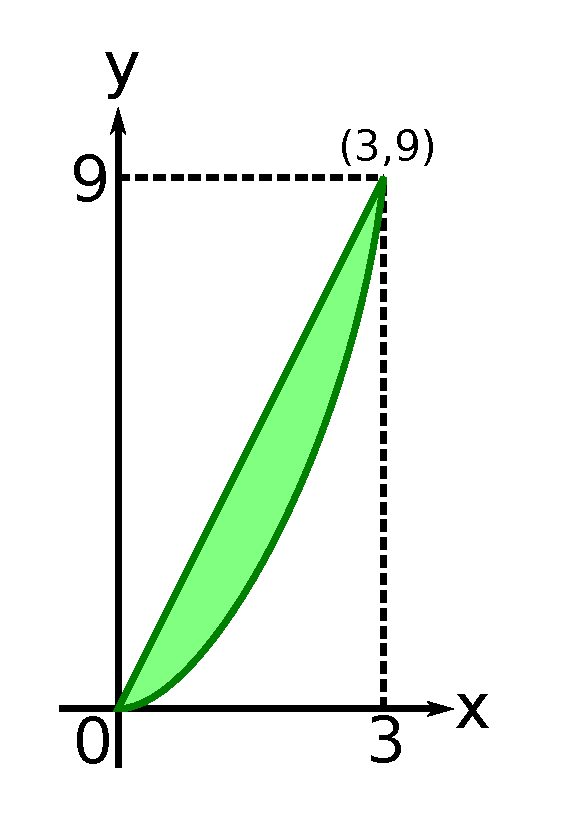
\includegraphics[height = 5cm]{Test_bench_part_3_images/Test_bench_part_3_image_5}}
\end{tabular}



%%%%%%%%%%%%%% QUESTION 4
\section*{Question 4:}

\begin{tabular}{cc}
\parbox{0.6\textwidth}{For the parabolic region \(\sigma\) on the right, express \(\sigma\) as: a Type I Cartesian region; a Type II Cartesian region; and a Polar region. In addition, given an arbitrary function \(f(x,y)\), or \(f(r,\theta)\) in polar coordinates, express the double integral \(\iint_{\sigma} f(x,y)dA\) as a nested (iterated) integral using each of the 3 different forms of \(\sigma\). Lastly, choose one of the 3 forms to compute the double integral \(\iint_{\sigma} \frac{dA}{x}\).}
& 
\parbox{0.4\textwidth}{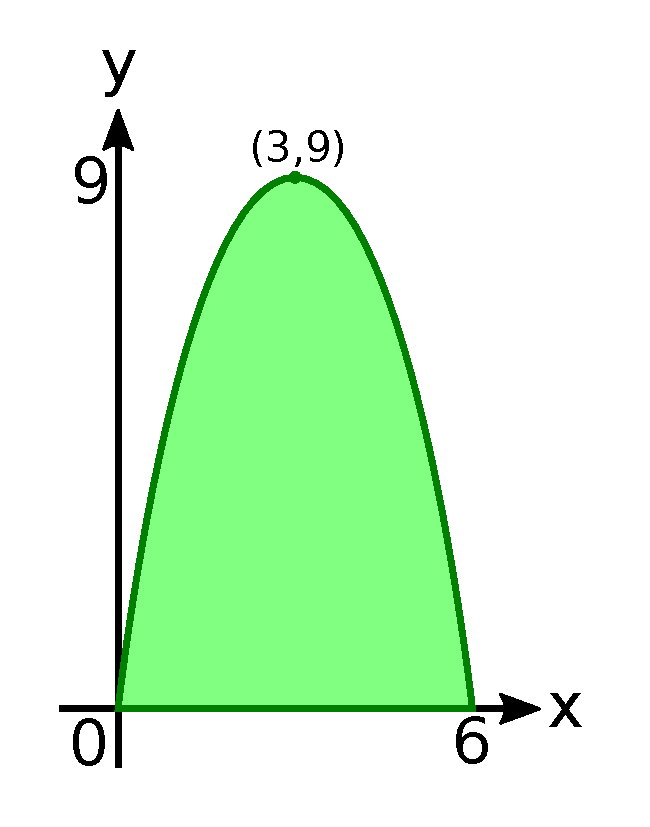
\includegraphics[height = 5cm]{Test_bench_part_3_images/Test_bench_part_3_image_1}}
\end{tabular}



%%%%%%%%%%%%%% QUESTION 5
\section*{Question 5:}

\begin{tabular}{cc}
\parbox{0.6\textwidth}{For the circular region \(\sigma\) on the right, express \(\sigma\) as a polar region, and then express the double integral \(\iint_{\sigma} f(r,\theta)dA\) as a nested integral. Lastly, evaluate the double integral \(\iint_{\sigma} \frac{\sqrt{\sin(2\theta)} \cdot dA}{r}\).} 
&
\parbox{0.4\textwidth}{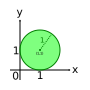
\includegraphics[width = 0.4\textwidth]{Test_bench_part_3_images/Test_bench_part_3_image_2}}
\end{tabular}



%%%%%%%%%%%%%% QUESTION 6
\section*{Question 6:}

Given the polar nested integral:
\[\int_{\theta = -\atan(2)}^{\pi/4}\int_{r = 0}^{\frac{2\cos\theta + \sin\theta}{\cos^2\theta}} r^2\cos\theta dr d\theta\]
Sketch the region covered by this double integral, convert it to Cartesian coordinates, and lastly evaluate the integral.



%%%%%%%%%%%%%% QUESTION 7
\section*{Question 7:}

Given the polar nested integral:
\[\int_{\theta = 0}^{\pi/2}\int_{r = 0}^{\frac{6}{2\cos\theta + 3\sin\theta}} r^2\cos\theta dr d\theta\]
Sketch the region covered by this double integral, convert it to Cartesian coordinates, and lastly evaluate the integral.



%%%%%%%%%%%%%% QUESTION 8
\section*{Question 8:}

Given the Cartesian nested integral:
\[\int_{x = -2}^2 \int_{y = 0}^{\sqrt{4-x^2}} y\sqrt{x^2 + y^2} \cdot dydx\]
Evaluate this integral directly, and then convert this integral to polar coordinates and evaluate that integral to demonstrate that you get the same result.



%%%%%%%%%%%%%% QUESTION 9
\section*{Question 9:}

Compute the volume between the two surfaces \(z_1(r,\theta) = \sqrt{R^2 - r^2}\) and \(z_2(r,\theta) = -\sqrt{R^2 - r^2}\) over the region \(\sigma = \{(r,\theta)|0 \leq \theta \leq 2\pi \;\text{and}\; 0 \leq r \leq R\}\) where \(R > 0\) is a fixed constant. What is the significance of this volume?



%%%%%%%%%%%%%% QUESTION 10
\section*{Question 10:}

Given the volume \(\Omega = \{(x,y,z)|0 \leq x \leq 1 \;\text{and}\; 0 \leq y \leq 2x \;\text{and}\; 0 \leq z \leq 3y\}\), compute the triple integral: 
\[\iiint_{\Omega} xyz dV\]



%%%%%%%%%%%%%% QUESTION 11
\section*{Question 11:}

\begin{tabular}{cc}
\parbox{0.6\textwidth}{For the tetrahedron \(\Omega\) on the right, compute the center of mass assuming a uniform mass density \(m\). The center of mass is the weighted average position \(\rowvec{x}{y}{z}\) of the points in \(\Omega\) where the ``weight" assigned to each point is the density: \[\mathbf{r}_{\text{CM}} = \frac{\iiint_{\Omega} m\rowvec{x}{y}{z}dV}{\iiint_{\Omega} mdV} = \frac{\iiint_{\Omega} \rowvec{x}{y}{z}dV}{\iiint_{\Omega} dV}\]} 
&
\parbox{0.4\textwidth}{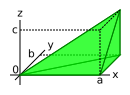
\includegraphics[width = 0.4\textwidth]{Test_bench_part_3_images/Test_bench_part_3_image_4}}
\end{tabular}






\end{document}









